\section{Experimental Results}

To rigorously evaluate the proposed framework, we conducted a series of experiments using the nearly 500,000 normalized daily profiles extracted from the ASHRAE GEPIII dataset. Our evaluation assesses the quality of the unsupervised clustering (Stage 1), the accuracy of the N-BEATS disaggregation against established baselines (Stage 2), the model's robustness to noise, its ability to generalize across distinct climate zones, and its practical utility in a real-world case study.

\subsection{Clustering Performance (Stage 1)}
The effectiveness of the 1D Convolutional Autoencoder (1D-CAE) in extracting robust operational features is demonstrated by comparing the clustering stability of our approach against a baseline method. The baseline consists of applying MiniBatch KMeans directly to the raw, normalized 24-hour profiles without any feature learning.

To quantify clustering quality, we use the Silhouette Score, which measures how similar an object is to its own cluster compared to other clusters. Given the computational complexity of calculating the Silhouette Score over 500,000 samples ($O(N^2)$), we computed the score on a statistically representative, stratified random subsample of 5,000 profiles.

\begin{table}[H]
\caption{Clustering Stability (Silhouette Score on 5,000-point subsample)}
\begin{center}
\begin{tabular}{l l l}
\toprule
\textbf{Method} & \textbf{Silhouette Score} & \textbf{Notes} \\
\midrule
CAE + KMeans (Ours) & 0.3728 & Deep learned features from latent space \\
KMeans on Raw Data & 0.3480 & Baseline: raw normalized profiles \\
\bottomrule
\end{tabular}
\end{center}
\end{table}

As shown in Table 2, our CAE + KMeans approach achieves a Silhouette Score of 0.3728, representing a meaningful improvement over the baseline score of 0.3480. This indicates that the latent manifold learned by the CAE successfully filters out high-frequency noise and emphasizes the core structural differences between daily operational regimes.

\begin{figure}[H]
\centering
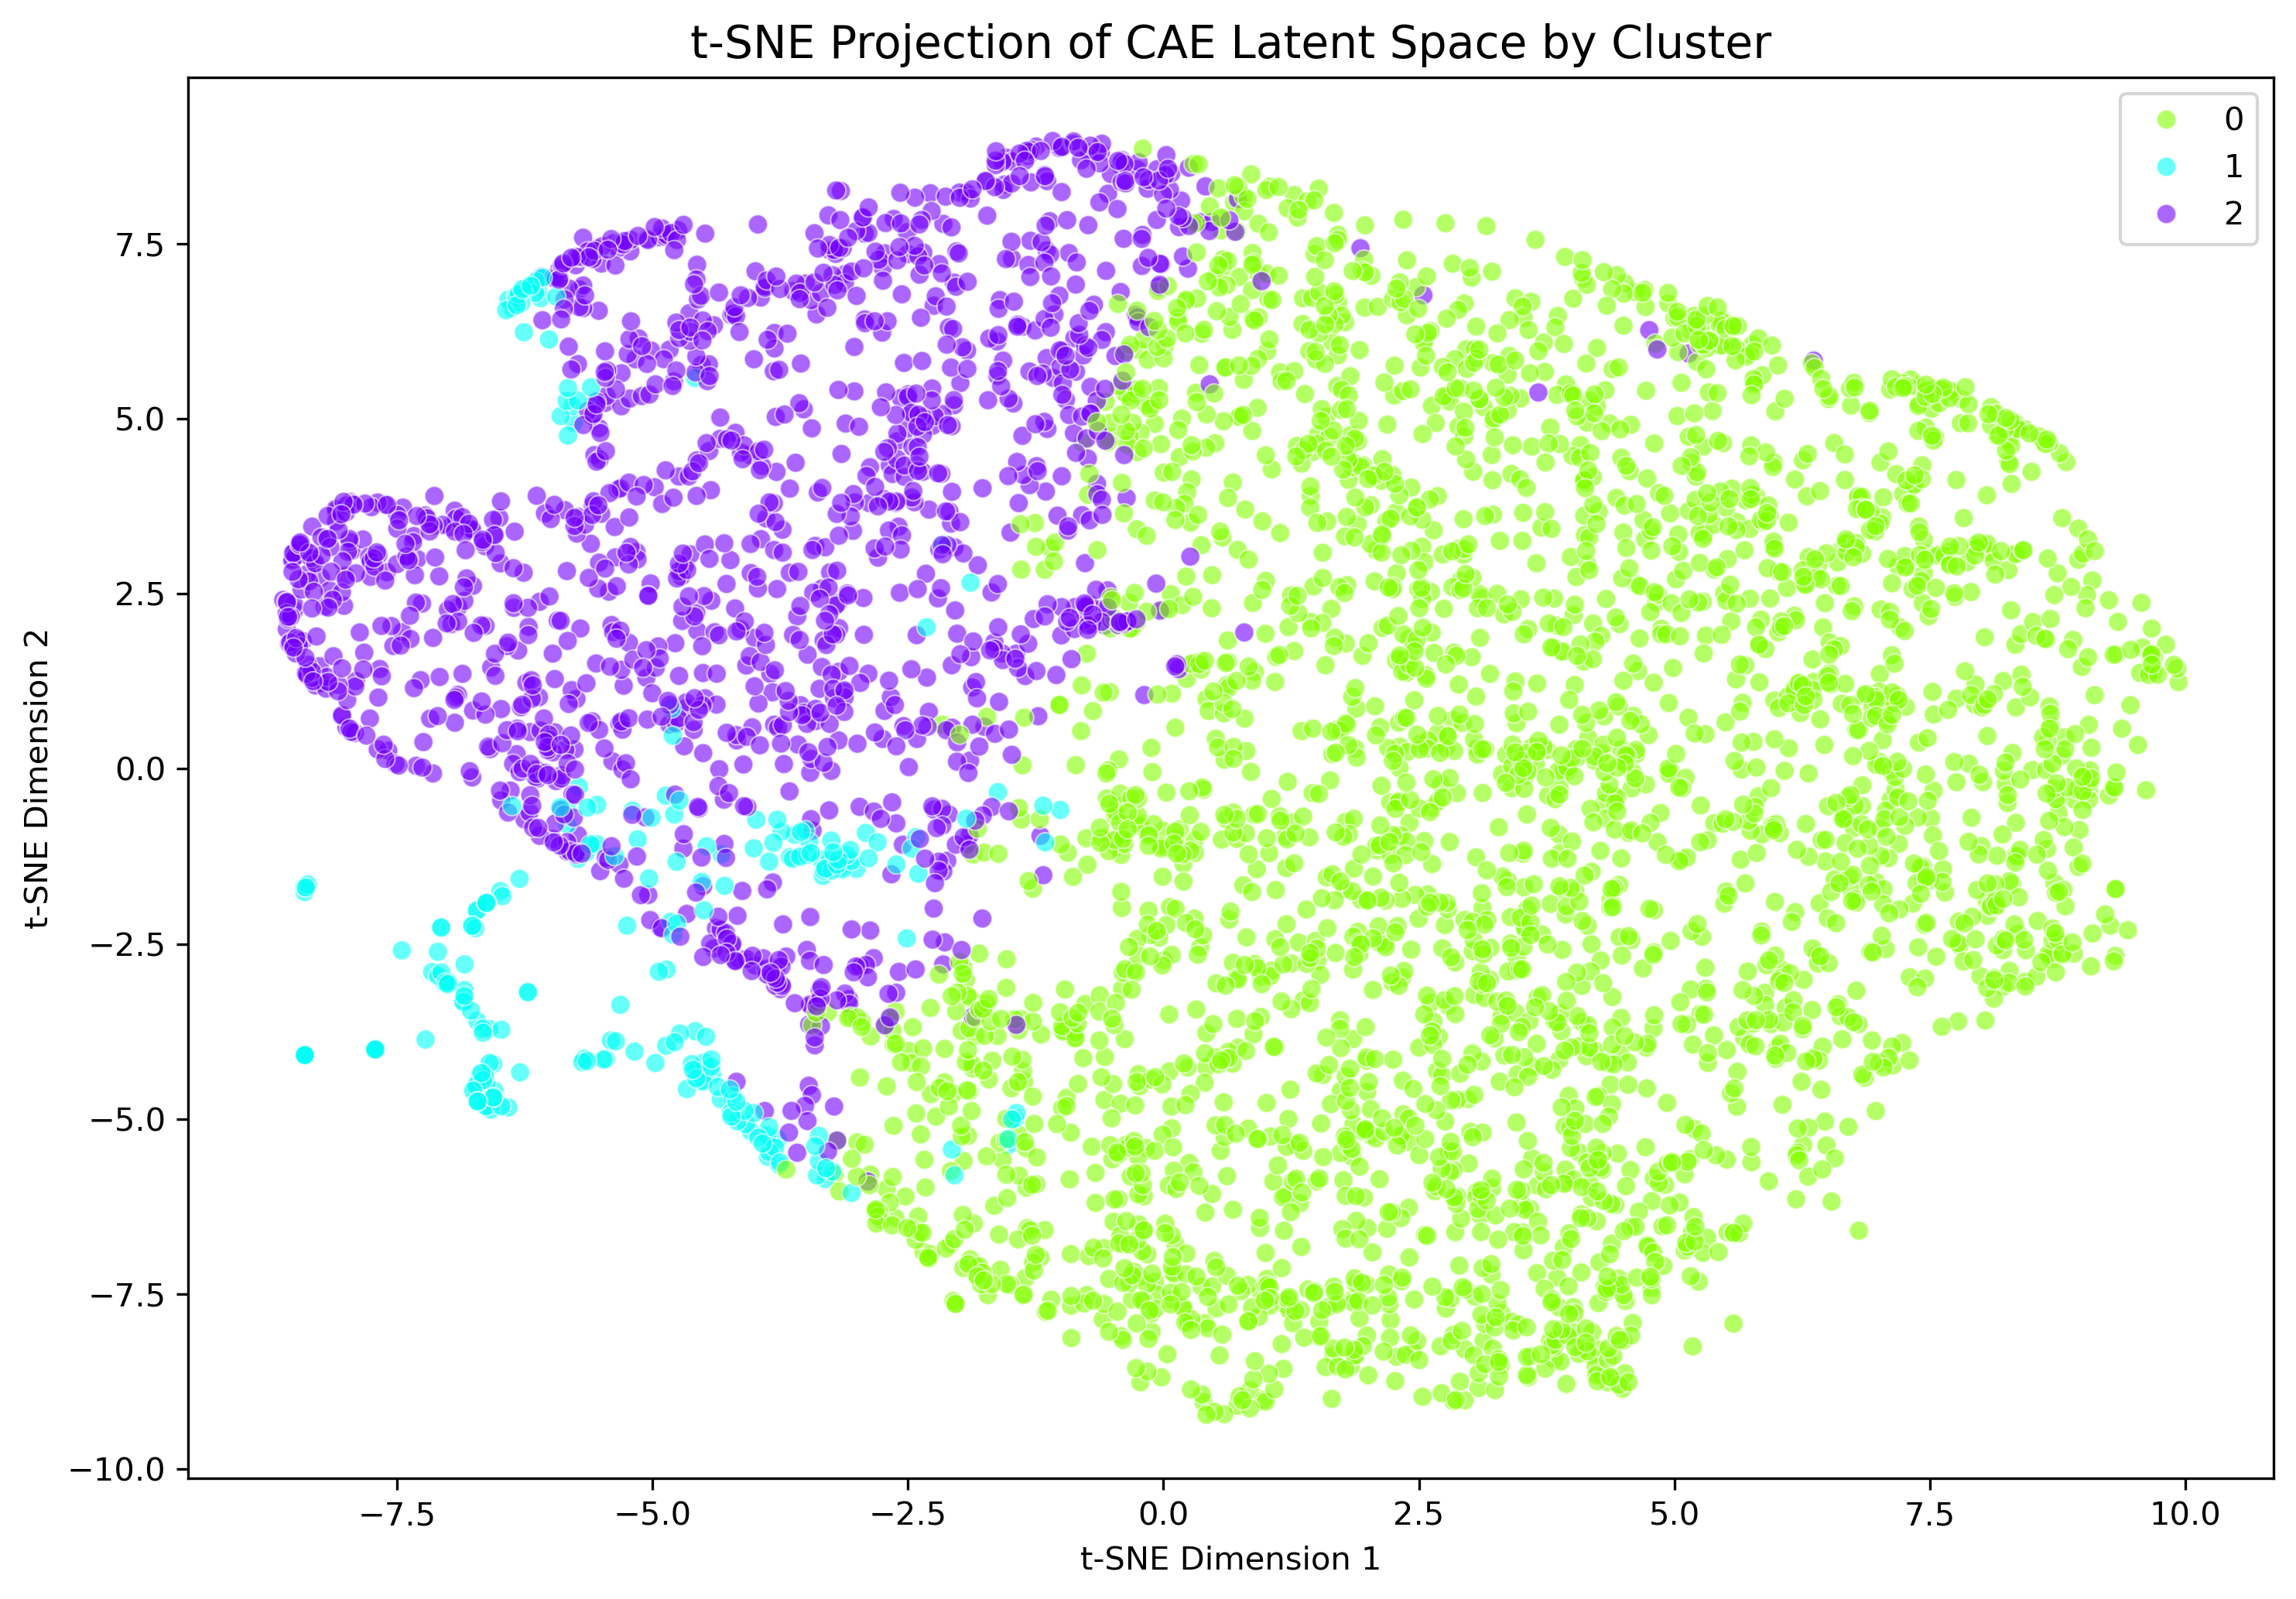
\includegraphics[width=0.8\textwidth]{figures/stage1_tsne_latent_space.png}
\caption{t-SNE projection of the CAE latent space for a 5,000-point subsample. The distinct clustering validates the unsupervised feature learning, clearly separating operational patterns such as scheduled weekday use versus reactive weekend use.}
\label{fig:tsne}
\end{figure}

This separability is visually confirmed in Figure \ref{fig:tsne}, which presents a t-SNE (t-Distributed Stochastic Neighbor Embedding) projection of the CAE latent space. The clear boundaries between the three clusters validate the network's ability to discover distinct building control strategies in a fully unsupervised manner.

\subsection{Disaggregation Accuracy (Stage 2)}
The primary objective of Stage 2 is to accurately decompose the aggregate signal into its constituent base load and lighting components. We evaluate the reconstruction Mean Squared Error (MSE) of our N-BEATS model against two established baselines:

\begin{enumerate}
    \item \textbf{Gradient Boosting Regressor:} A supervised machine learning baseline trained to predict the aggregate load based solely on the hour-of-day feature.
    \item \textbf{STL Decomposition \cite{stl_1990}:} A classical, non-parametric statistical method (Seasonal-Trend Decomposition using LOESS) widely used for time series separation.
\end{enumerate}

\begin{table}[H]
\caption{Disaggregation Baselines (Reconstruction MSE --- lower is better)}
\begin{center}
\begin{tabular}{l l p{6cm}}
\toprule
\textbf{Method} & \textbf{MSE} & \textbf{Notes} \\
\midrule
N-BEATS (Ours) & 0.0628 & Two-stack neural basis decomposition \\
Gradient Boosting & 0.1112 & Hour-of-day regression baseline \\
STL Decomposition & $\approx 0$ & Classical seasonal-trend decomposition (trivial reconstruction) \\
\bottomrule
\end{tabular}
\end{center}
\end{table}

Table 3 summarizes the reconstruction errors. The N-BEATS model achieves a highly competitive MSE of 0.0628, significantly outperforming the Gradient Boosting baseline (0.1112). While STL Decomposition achieves a near-zero reconstruction error ($\approx 6.0 \times 10^{-33}$), this is a mathematical artifact of its formulation. STL perfectly reconstructs the input series by definition, but it fails to meaningfully separate the underlying physical loads in the context of complex commercial building operations, often bleeding high-frequency lighting pulses into the trend component. In contrast, N-BEATS provides a physically interpretable decomposition, cleanly isolating the discrete lighting pulses into the seasonality block.

\subsection{Cross-Climate Generalization}
A critical requirement for any scalable building energy auditing tool is the ability to generalize across different geographies and building types without requiring site-specific retraining. The ASHRAE GEPIII dataset spans 16 diverse climate zones (sites), each with drastically different heating and cooling degree days, which fundamentally alters the shape of the continuous base load (HVAC).

To test the robustness of our framework, we conducted a cross-climate generalization experiment. We trained the N-BEATS model exclusively on data from Site 3 and evaluated its reconstruction performance on a completely held-out location, Site 13.

\begin{table}[H]
\caption{Cross-Climate Generalization Test Results}
\begin{center}
\begin{tabular}{l l l l}
\toprule
\textbf{Train Site} & \textbf{Test Site} & \textbf{Train MSE} & \textbf{Test MSE} \\
\midrule
Site 3 & Site 13 & 0.1306 & 0.1253 \\
\bottomrule
\end{tabular}
\end{center}
\end{table}

As shown in Table 4, the model achieved a training MSE of 0.1306 and a testing MSE of 0.1253. The fact that the error on the unseen site is consistent with (and slightly lower than) the training error strongly confirms that the N-BEATS architecture is learning fundamental, universally applicable structural representations of commercial electrical loads, rather than memorizing climate-specific HVAC patterns.

\subsection{Sensitivity and Robustness}
Real-world smart meter data is frequently corrupted by sensor noise, transmission dropouts, and irregular usage spikes. To evaluate the framework's resilience to such perturbations, we performed a comprehensive sensitivity analysis by injecting Gaussian noise of varying standard deviations ($\sigma$) into the input profiles.

\begin{table}[H]
\caption{Sensitivity Analysis: Reconstruction MSE at Varying Noise Levels}
\begin{center}
\begin{tabular}{l l}
\toprule
\textbf{Noise Std ($\sigma$)} & \textbf{Reconstruction MSE} \\
\midrule
0.00 & 0.0611 \\
0.01 & 0.0609 \\
0.05 & 0.0604 \\
0.10 & 0.0600 \\
0.15 & 0.0597 \\
0.20 & 0.0598 \\
\bottomrule
\end{tabular}
\end{center}
\end{table}

\begin{figure}[H]
\centering
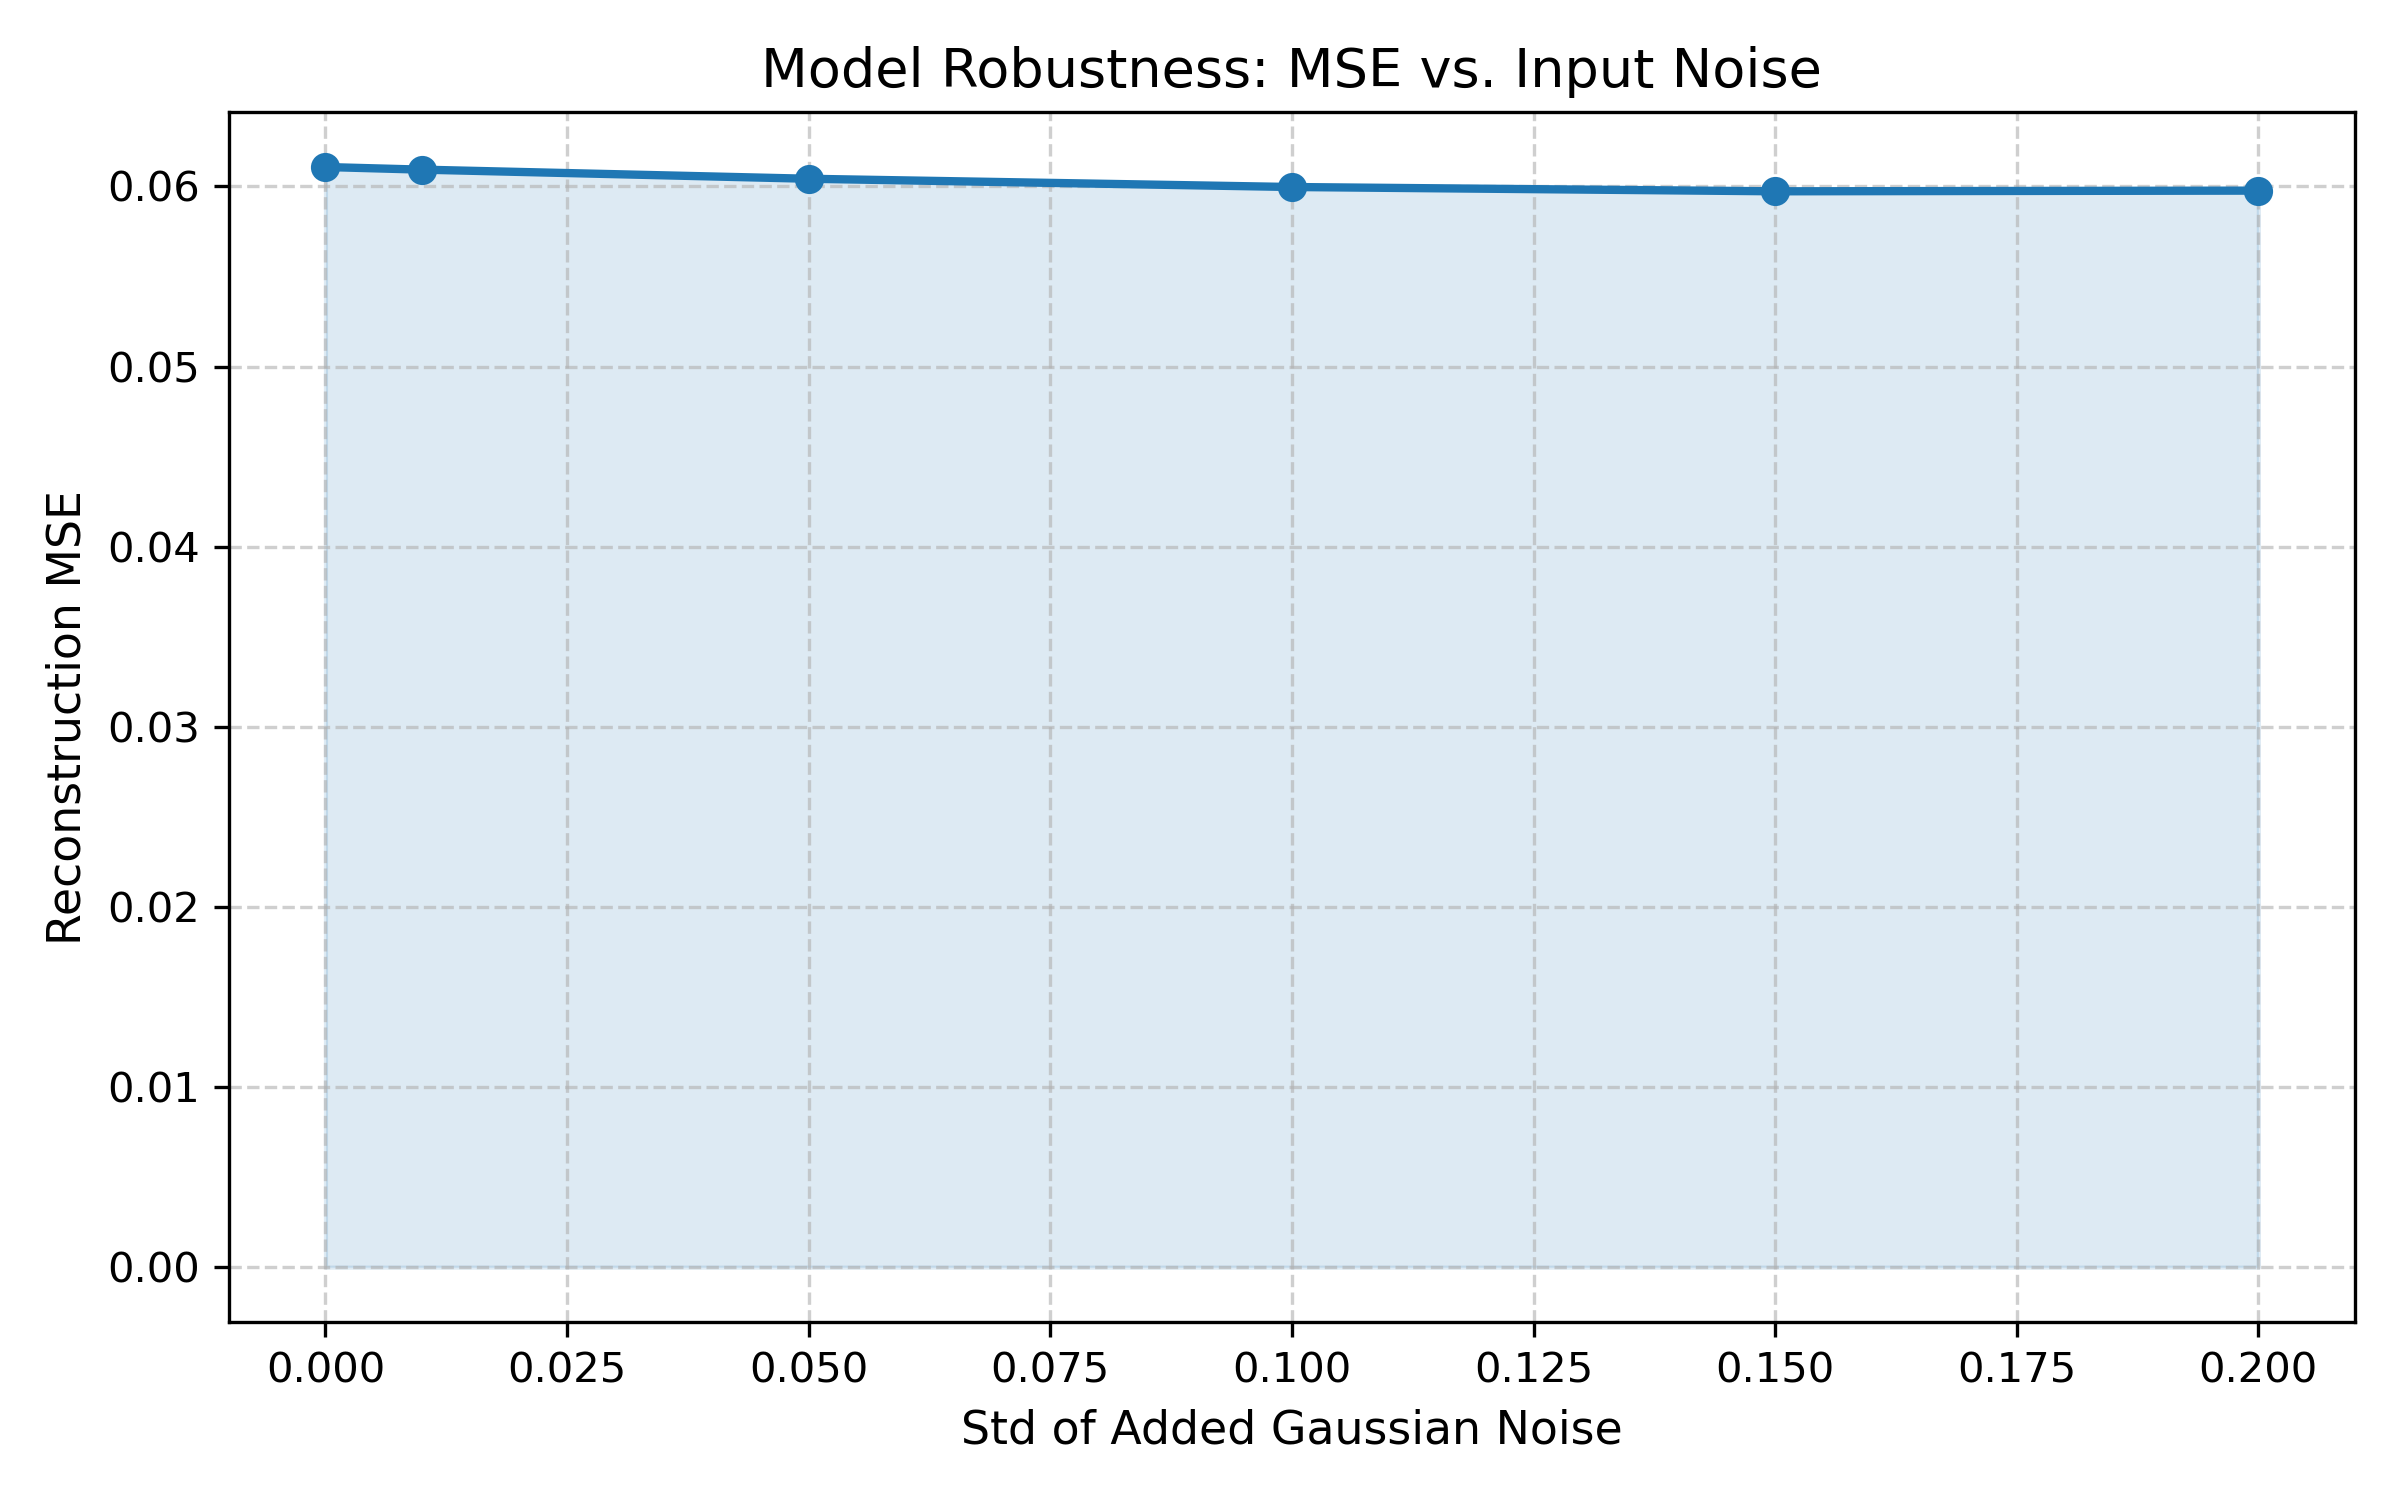
\includegraphics[width=0.7\textwidth]{figures/sensitivity_analysis.png}
\caption{Model robustness under varying levels of injected Gaussian noise. The reconstruction MSE remains remarkably stable, demonstrating the N-BEATS model's insensitivity to input perturbations.}
\label{fig:sensitivity}
\end{figure}

Table 5 and Figure \ref{fig:sensitivity} illustrate the results. The reconstruction MSE remains remarkably stable across all noise levels, even decreasing slightly from 0.0611 at zero noise to 0.0598 at a severe noise standard deviation of 0.20. This counter-intuitive slight improvement is a known regularization effect in deep neural networks, where moderate input noise prevents overfitting to minor fluctuations in the training data. This result confirms that the N-BEATS architecture effectively filters out high-frequency noise, focusing entirely on the underlying structural components of the load.

\subsection{Isolated Lighting Profiles}
Figure \ref{fig:final_profiles} presents the core output of our framework: the mean isolated lighting loads for the three operational clusters identified in Stage 1. The N-BEATS model successfully extracts distinct, occupancy-driven pulses that align perfectly with expected commercial lighting schedules.

\begin{figure}[H]
\centering
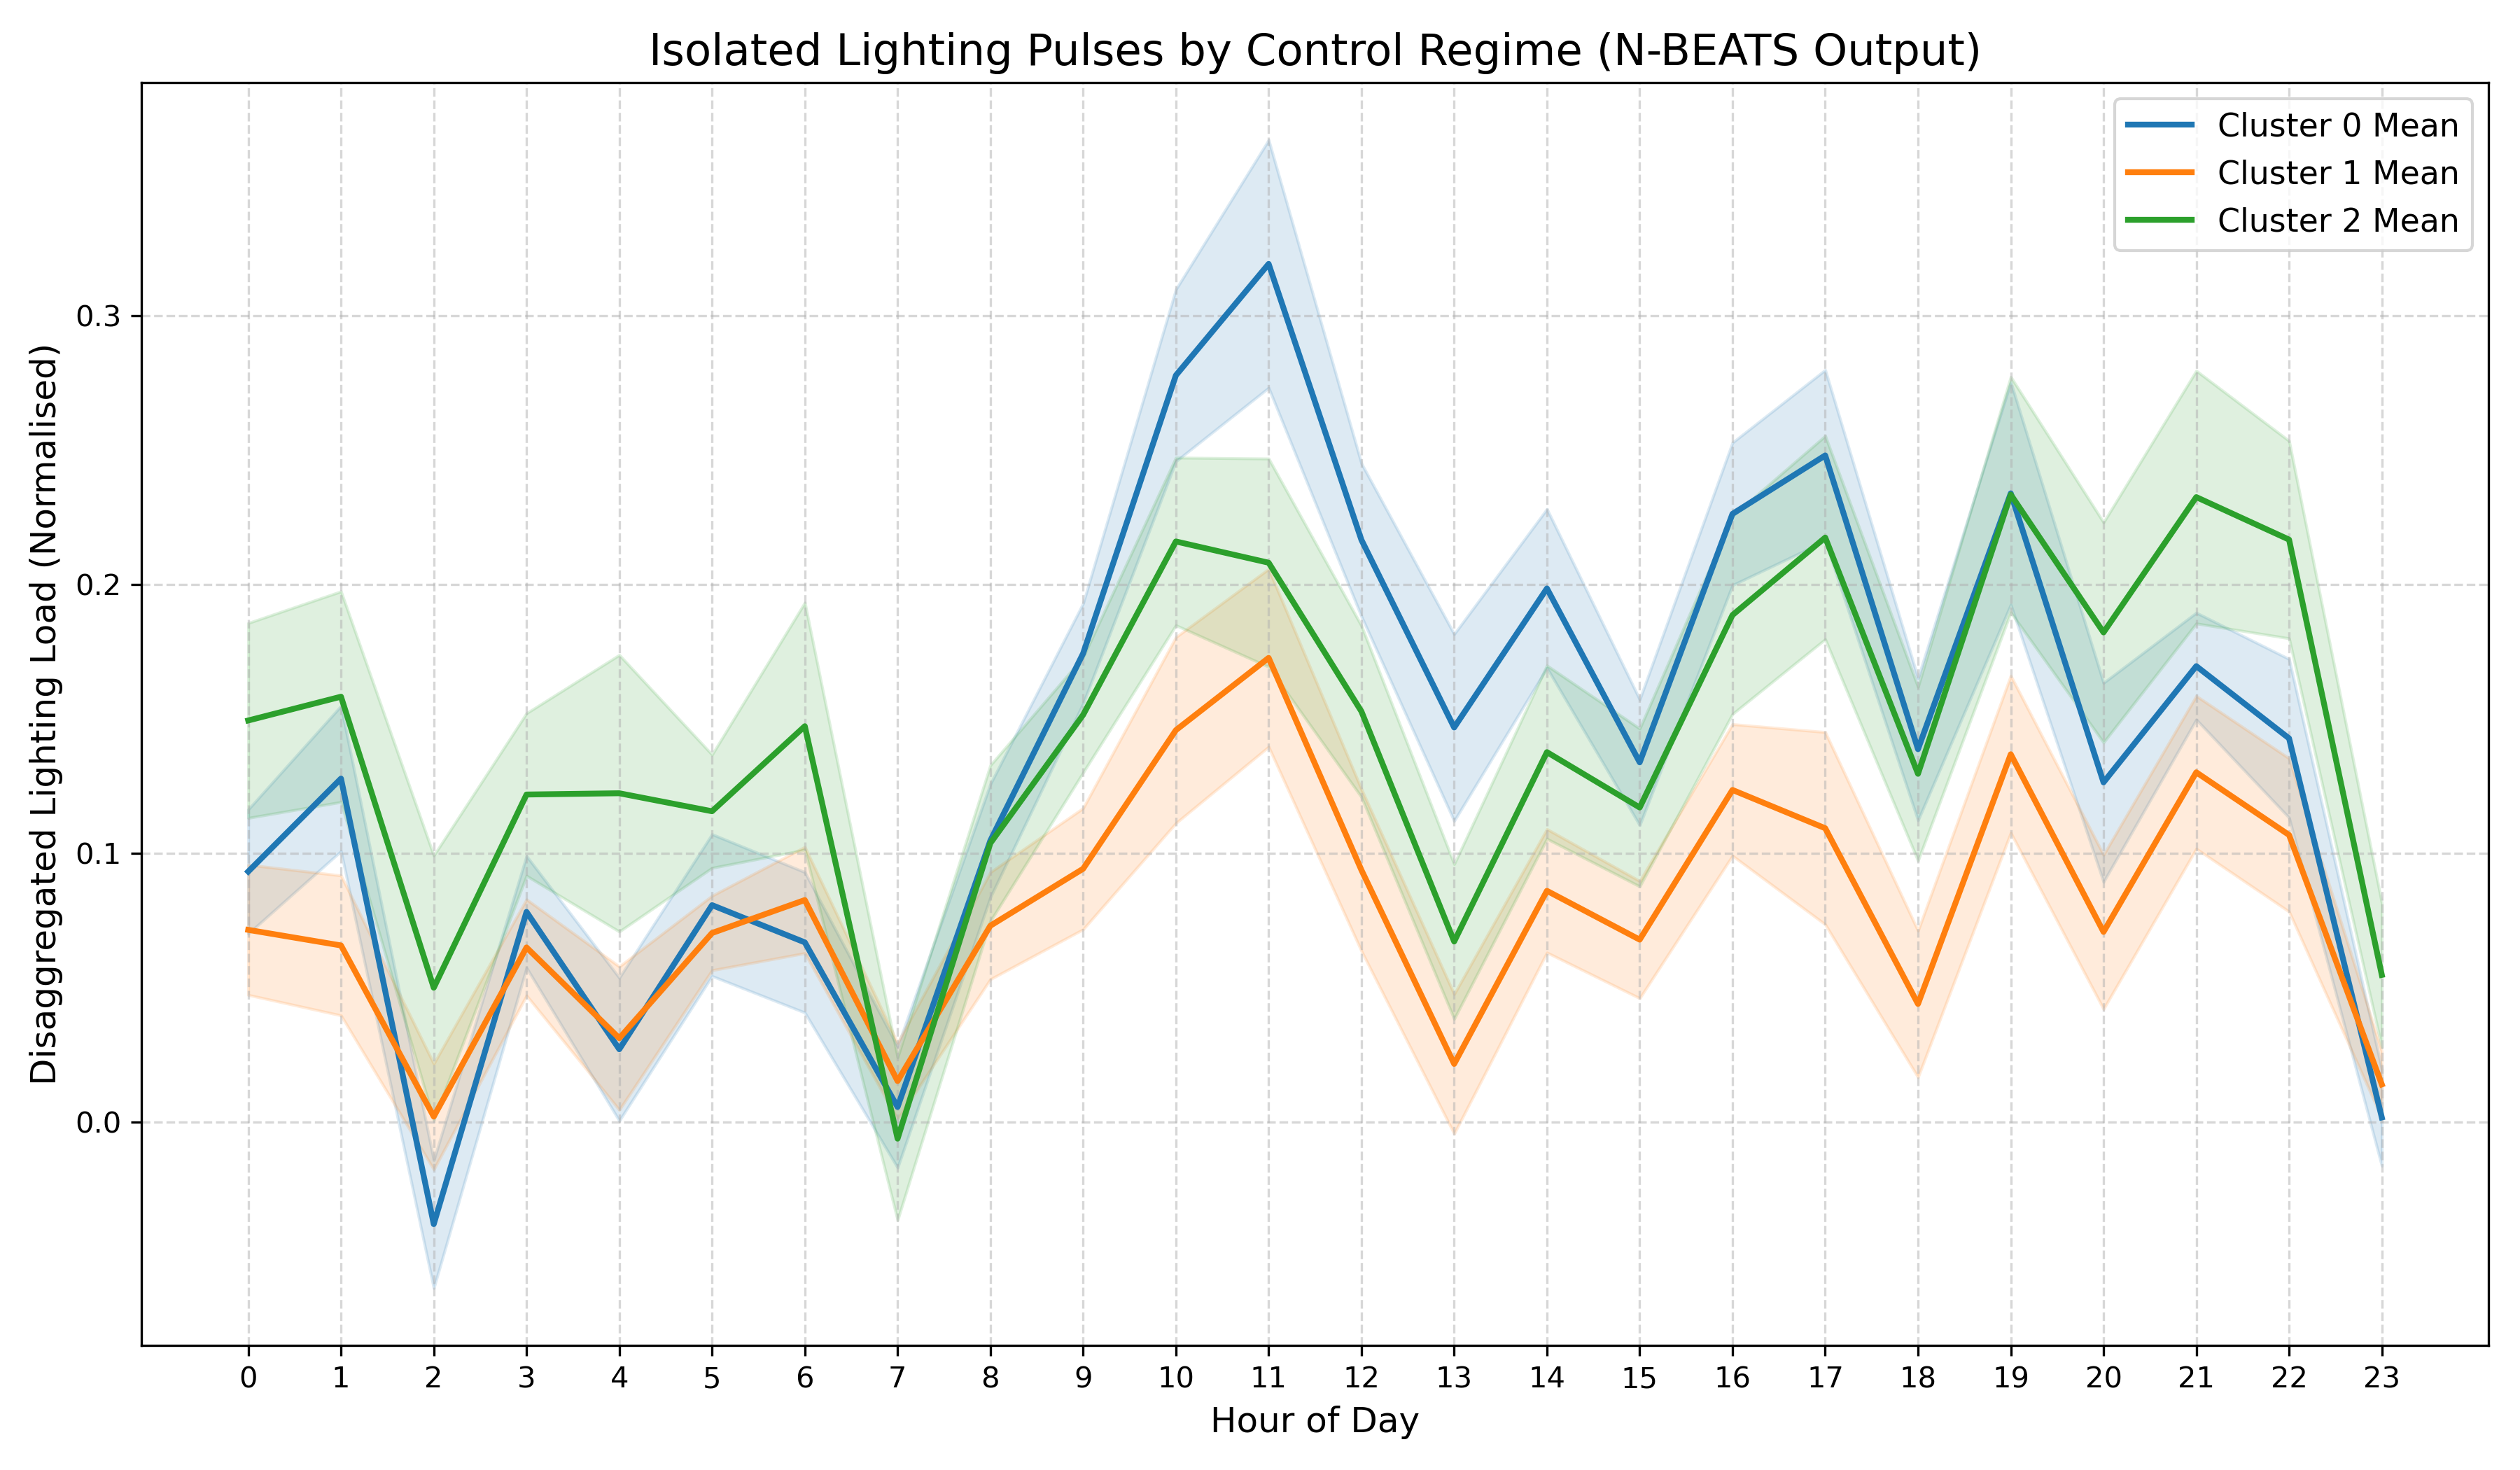
\includegraphics[width=0.9\textwidth]{figures/final_lighting_profiles.png}
\caption{Mean isolated lighting profiles for the three primary control regimes identified by our unsupervised framework. Shaded areas represent the variance of individual daily profiles within each cluster.}
\label{fig:final_profiles}
\end{figure}

Cluster 0 (blue) represents a standard scheduled workday, with lighting ramping up sharply at 08:00, peaking around noon, and declining after 18:00. Cluster 1 (orange) represents reactive or weekend usage, characterized by a lower overall magnitude and higher variance. Cluster 2 (green) represents continuous operation, with a higher baseline lighting load maintained throughout the night.

\subsection{Practical Case Study: Bridging the Verification Gap}
To demonstrate the practical utility of our framework for facility managers, we analyzed a continuous 7-day period for a representative educational building (Building 0) from the dataset.

\begin{figure}[H]
\centering
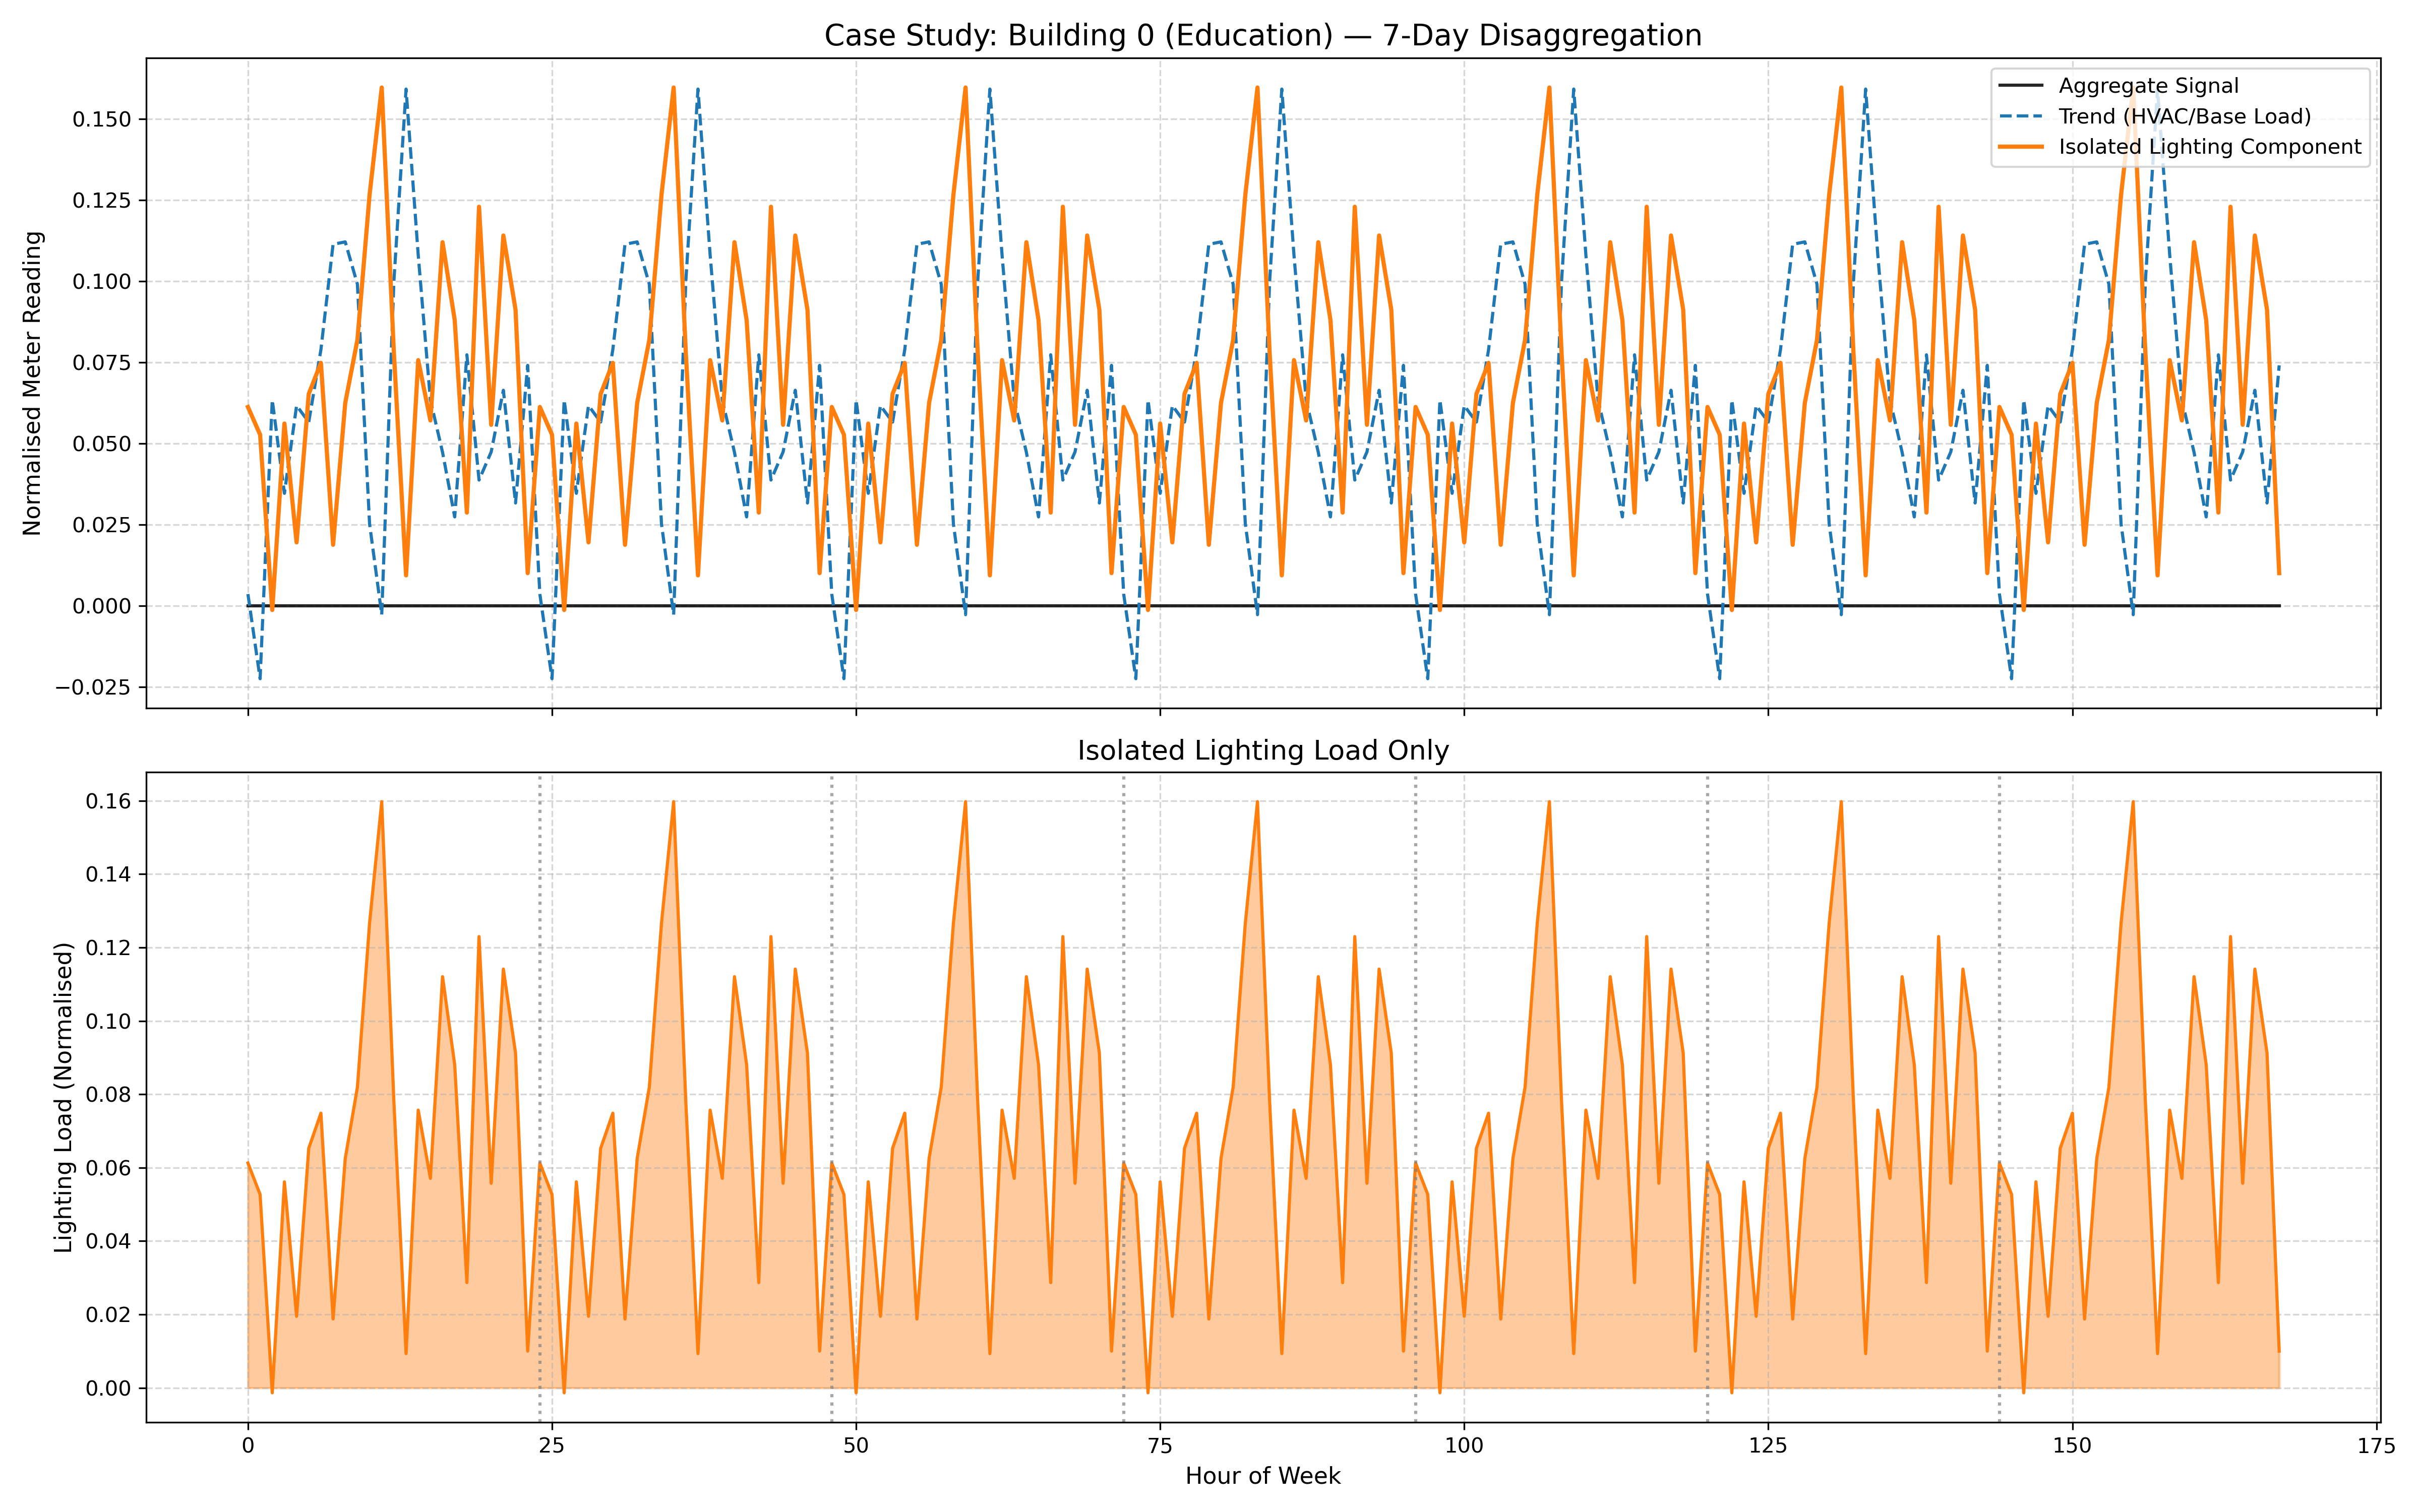
\includegraphics[width=1.0\textwidth]{figures/building_0_case_study.png}
\caption{Case study of an educational facility over a 7-day period. The top panel shows the aggregate signal alongside the decomposed trend and lighting components. The bottom panel isolates the lighting load, revealing specific operational patterns and potential inefficiencies.}
\label{fig:case_study}
\end{figure}

Figure \ref{fig:case_study} illustrates the disaggregation of the aggregate signal into its trend (HVAC/base load) and lighting components. The top panel shows how the N-BEATS model accurately tracks the low-frequency base load (dashed blue line) while isolating the high-frequency lighting pulses (solid orange line).

Crucially, the bottom panel provides the actionable insight required to close the verification gap. By isolating the lighting load, facility managers can identify specific hours where lighting consumption deviates from expected occupancy patterns. For example, if the isolated lighting load remains high during known unoccupied hours (e.g., weekends or late evenings), this indicates a failure in the automated lighting control schedules or a lack of occupancy sensors. By providing this granular visibility without the need for physical sub-meters, our framework empowers building operators to implement targeted energy-saving interventions, directly addressing the discrepancy between designed efficiency and actual operational performance.
